
En esta sección se explican los detalles implementativos de nuestro clasificador.

\subsection{Datos de Entrada}

El programa tiene el set de datos de MNIST ubicado en la carpeta $mnist$ en un archivo comprimido, este es convertido a archivos de texto que contienen un pixel por línea con un script de python el cual aloja los archivos en la carpeta $data$. Esto se hace para facilitar la posterior lectura de estos datos por nuestro programa.

Una vez hecho esto se puede utilizar program.py para compilar y ejecutar nuestro código de c que entrena una red neuronal para reconocer estos caracteres. Tanto en la carpeta $float$ como en la carpeta $double$ se encontrará el código que implementa dicho programa y las correspondientes herramientas de compilación. Para compilar los archivos fuente manualmente basta con utilizar el \texttt{Makefile}, este crea los archivos \texttt{asm\_version} y \texttt{c\_version} que ejecutan la red neuronal.

\subsection{Secciones Principales}

En las carpetas $double$ y $float$ hay versiones equivalentes del clasificador para estos dos tipos de datos.
\\
\\
Dentro de las carpetas hay 3 archivos con código fuente, $helpers$, $tensorOps$ y $nn$.
\\
\\
Los archivos $helpers$ implementan varias funciones útiles, entre otras cosas las que utilizamos para leer los TXTs donde estan los datos de entrenamiento, también algunas funciones matriciales básicas como transpocisión e impresión.
\\
\\
Luego esta $tensorOps$ en el cual pusimos los métodos que implementamos tanto en $C$ como en $ASSEMBLER$ estas son operaciones matriciales y vectoriales como el producto matricial y la suma vectorial. Es importante entender el objetivo de la implementación en $ASSEMBLER$, al utilizar SIMD podemos realizar 2 operaciones de $double$ a la vez y 4 de $float$, por ejemplo la suma, multiplicación y reordenamiento de valores en un registro. Esta herramienta nos permitirá paralelizar los cálculos e idealmente mejorar los tiempos significativamente.
\\
\\
Por último esta $nn$ que es el archivo que utiliza a los demás para implementar toda la lógica de la red neuronal y donde se encuentra el main de nuestro programa.

\subsection{Estructura de la Red Neuronal}

La estructura de la red implementada en los archivos $nn$ esta dada por una capa de entrada formada por 784 inputs ($28^2$) las cuales representan cada uno de los pixels de las imágenes. Esta capa se conecta a la capa interna de nuestra red y luego de ahí se va a la capa externa, formada por 10 salidas representando cada uno de los posibles digitos resultantes.
\\
\\
Por ejemplo, al ingresar los valores de una imagen que represente al número 2 se esperará que la tercera neurona de salida (Ya que se empieza a contar desde el cero) indique 1 y todas las demas outputs indiquen 0.

\begin{figure}[H]
\fcolorbox{black}{black}{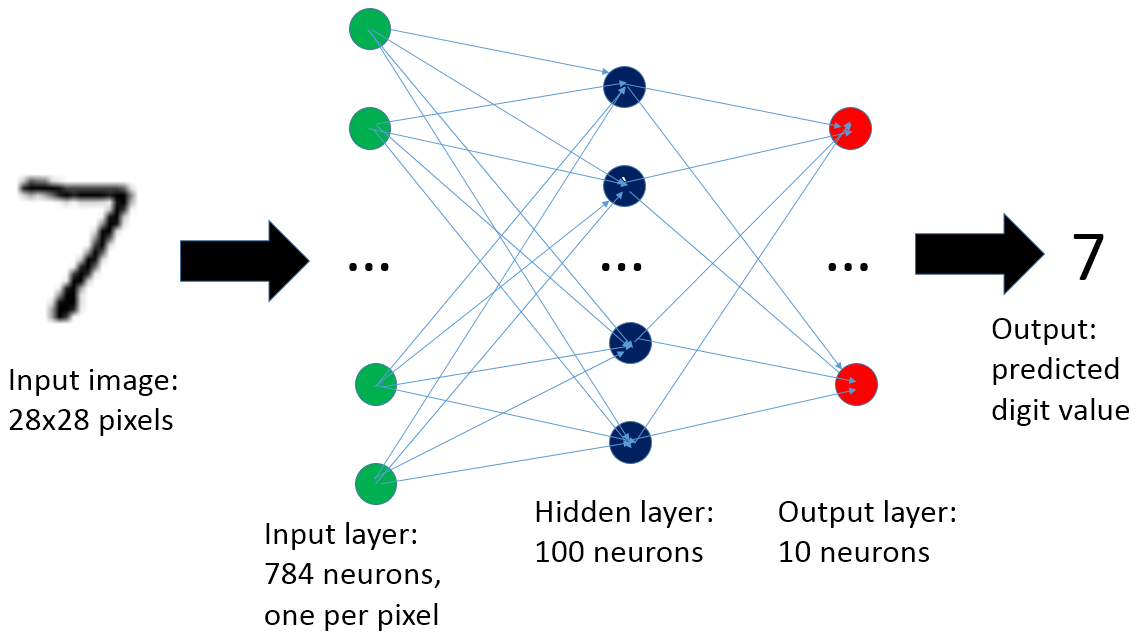
\includegraphics[width=0.9\linewidth]{imgs/MNIST_neuralnet.png}}
\centering
\caption{Diagrama de la red implementada}
\centering
\end{figure}

Es importante notar que si bien la cantidad de neuronas en la capa interna y externa esta fijada por el dominio del problema, la cantidad de neuronas en la capa oculta es una variable con la que se puede jugar, en la imagen se ve el caso en que se utilizan 100 neuronas como capa interna pero nosotros utilizamos 30 para la mayor parte de la experimentación ya que con este valor obtuvimos un buen trade-off entre tiempo de cómputo y performance.

\subsection{Métodos implementados Assembler}

A continuación damos una breve explicación de los métodos que implementamos en $ASSEMBLER$ para intentar mejorar la performance. Todos ellos poseen la propiedad de realizar cierta operación aritmética repetidas veces para distintos valores, haciendo propicio el intento de paralelización con SIMD.

\subsubsection{cost\_derivative}

Este método es el gradiente del error cuadrático medio lo cual se reduce simplemente al cómputo de la resta entre vectores.
\\
\\
\begin{lstlisting}
void cost_derivative(double* res_vec, double* target_mat, uint cant_imgs, double* output) {
  for (int i = 0; i < 10; i++) {
    for (uint j = 0; j < cant_imgs; j++){
        output[i * cant_imgs + j] = res_vec[i * cant_imgs + j] - target_mat[i * cant_imgs + j];
    }
  }
}
\end{lstlisting}

\subsubsection{vector\_sum}

Como indica su nombre esta método computa la suma vectorial.
\\
\\
\begin{lstlisting}[frame=single]
void vector_sum(double* vector1, double* vector2, uint n, double* output){
  for (int i = 0; i < n; i++) {
    output[i] = vector1[i] + vector2[i];
  }
}
\end{lstlisting}


\subsubsection{update\_weight}

Esta función actualiza los valores de un vector restandole un porcentaje de los valores de otro vector. El porcentaje descontado esta dado por la variable c. Esto se utiliza en la red neuronal para ir actualizando los parámetros de las neuronas hasta que converjan a una configuración que clasifica lo mejor posible.
\\
\\
\begin{lstlisting}[frame=single]
void update_weight(double* w, double* nw, uint w_size, double c){
  for(uint i = 0; i < w_size; i++){
    w[i] -= c * nw[i];
  }
}
\end{lstlisting}

\subsubsection{hadamard\_product}

El producto de Hadamard consiste en la multiplicación componente a componente entre dos matrices.
\\
\\
\begin{lstlisting}[frame=single]
void hadamard_product(double* matrix1, double* matrix2, uint n, uint m, double* output){
  for(uint i = 0; i < n; i++){
    for(uint j = 0; j < m; j++){
      output[i * m + j] = matrix1[i * m + j] * matrix2[i * m + j];
    }
  }
}
\end{lstlisting}

\subsubsection{matrix\_prod}

Este es el clásico producto matricial donde $matrix1$ es de $n \times m$, $matrix2$ es de $m \times l$ y la variable de salida, $output$, de dimensiones $n \times l$.
\\
\\
\begin{lstlisting}[frame=single,xleftmargin=1cm]
void matrix_prod(double* matrix1, double* matrix2, uint n, uint m, uint l, double* output){
  for(uint i = 0; i < n; i++) {
    for(uint j = 0; j < l; j++){
      output[i * l + j] = 0;
      for(uint k = 0; k < m; k++){
        output[i * l + j] += matrix1[i * m + k] * matrix2[k * l + j];
      }
    }
  }
}
\end{lstlisting}


\subsection{Tests}

Tanto la versión del programa que utiliza Floats como la que utiliza Doubles tienen un conjunto de tests en las funciones que implementamos en ASSEMBLER y C, esto fue para corroborar el buen funcionamiento de lo desarrollado y ayudarnos a debuguear.
\\
\\
Dichos tests se encuentran en la carpeta $test$ y se compilan con el \texttt{Makefile} el cual crea el ejecutable $test$ que corre los mismos.